\section*{Results}


With two axes, axis evolution followed patterns associated with the type 
of tradeoff the two axes had when evolved together
(i.e., with the value of $\eta$)
(Figure \ref{fig:two-axis-outcomes}).
When the tradeoff is sub-additive ($\eta = -0.6$), there is a single
stable point in the axis space, where both axes are
maximized---within the limits imposed by axes' negative effects on 
the growth rate.
When the tradeoff is super-additive ($\eta = 0.6$), there are two
alternative stable states, one for each axis being maximized while the 
other is zero.
Lastly, when the tradeoff is additive ($\eta = 0$), axes
evolve to any point on a neutrally stable ring.
The locations of these states are determined by 
the baseline growth rate, 
the cost of increasing axes on the growth rate,
and, when $\eta \ne 0$, the non-additive tradeoff
(Equations \ref{eq:two-axes-finals-eta-negative},
\ref{eq:two-axes-finals-eta-zero}, and 
\ref{eq:two-axes-finals-eta-positive} for 
$\eta < 0$, $\eta = 0$, and $\eta > 0$, respectively).

\begin{figure}[ht!]
\centering
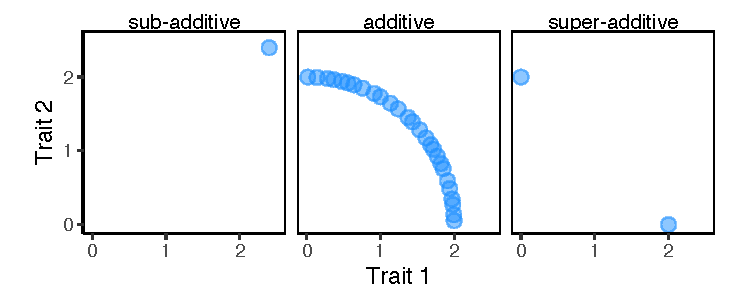
\includegraphics{1-outcomes_q2.pdf}
\caption{Unique axis values for surviving species in simulations of 2-axis communities,
    for tradeoffs being sub-additive ($\eta < 0$), additive ($\eta = 0$), or 
    super-additive ($\eta > 0$).}
\label{fig:two-axis-outcomes}
\end{figure}


The proportion of the 100 species introduced to communities that survived and
coexisted depended on the additive genetic variance, 
the tradeoffs, and
how conflicting / non-conflicting evolution was (i.e., the values in $\mathbf{d}$)
(Figure \ref{fig:coexistence-spp}A).
Increasing values of $\mathbf{d}$ (where all values in the vector are equal)
caused greater number of species to coexist
because species evolving toward a fitness peak benefited rather than 
harmed other species with high $\mathbf{d}$.
This pattern was least obvious with additive tradeoffs.
There was an abrupt change when evolution was conflicting for both axes 
(i.e., $\mathbf{d} < 0$), where only one species ever survived.
Greater additive genetic variance monotonically increased the proportion of 
surviving species, via an increased probability 
of evolutionary rescue: When genetic variance was high, 
species could often evolve quickly enough towards a 
fitness peak to prevent themselves from going extinct.
The greatest number of surviving species occurred with additive tradeoffs
because each new community member had only to evolve to anywhere along the
neutrally stable ring to survive, rather than to one or two distinct points.
Sub-additive tradeoffs resulted in greater numbers of species than super-additive
because the lower cost of evolving multiple axes caused species to evolve
high values of both axes.
When combined with non-conflicting evolution,
this decreased competition experienced by all species, both on a 
per-capita basis (the term $- \mathbf{v}_{j}^{\text{T}} \mathbf{D} \mathbf{v}_j$ 
in equation \ref{eq:competition})
and overall (because all $N_j$ are greater).



When we kept evolution for the second axis non-conflicting ($d_2 = 0.1$) and
adjusted evolution for axis 1, the results were slightly more complicated
(Figure \ref{fig:coexistence-spp}B).
Additive genetic variance had a similar effect as when we varied both axes' evolution.
The effect of varying $d_1$, however, depended on the tradeoffs.
With sub-additive tradeoffs, the threshold for coexistence was $d_1 = -0.1$.
This is because species evolve to maximize both axes, so $d_1 + d_2$
determined the coexistence behavior of the community.
When tradeoffs are additive or super-additive, $\min (d_1, d_2)$ determined whether 
coexistence could occur.
Under super-additivity, this occurs because species evolve to maximize one axis while
the other evolves to zero.
When one $d$ is negative, if sufficient species are added to the community and 
each starts with random axis values, 
one will inevitably evolve to maximize the axis that is conflicting. 
That species will exclude all others.
A similar dynamic occurs when tradeoffs are additive, except that
the excluding species evolves to be near, rather than exactly on, 
the conflicting axis being maximized.


\begin{figure}[ht!]
\centering
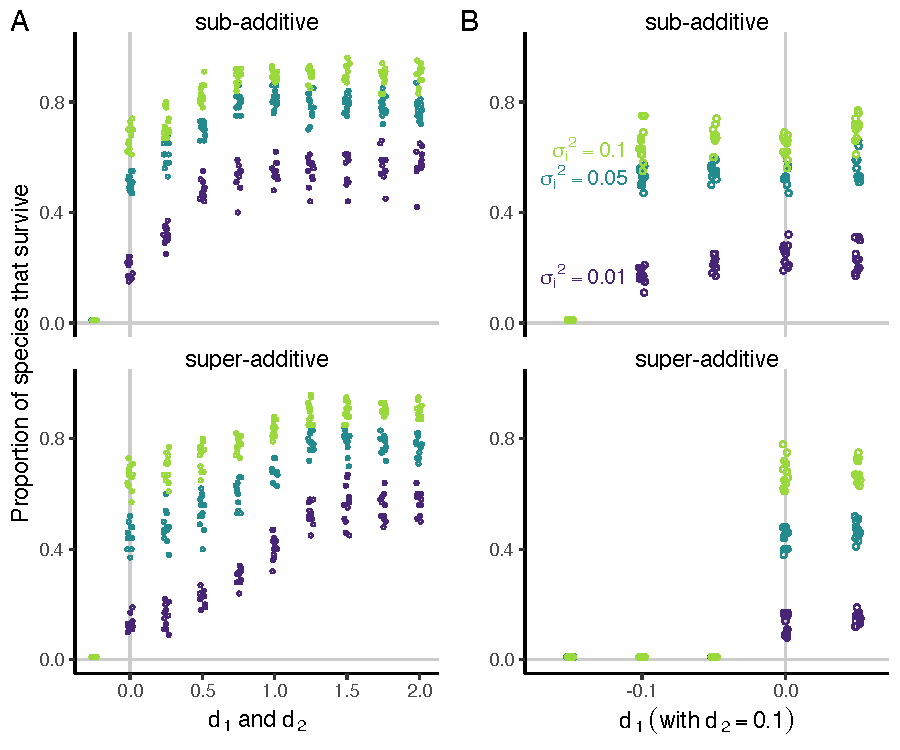
\includegraphics{2-coexist_spp.pdf}
\caption{Proportion of species that survived in simulations of 100-species, 2-axis
    communities with varying additive genetic variances ($\sigma_i^2$), and 
    varying (A) $d_1$ and $d_2$ or (B) varying $d_1$ with $d_2$ fixed at 0.1.
    Shown for sub-additive ($\eta < 0$), additive ($\eta = 0$), and 
    super-additive ($\eta > 0$) tradeoffs.}
\label{fig:coexistence-spp}
\end{figure}


We also ran some of these simulations with varying levels of stochasticity
in the population dynamics and axis evolution.
Stochasticity had particularly strong negative effects on the proportion
of species surviving at low values of $d_1$ and $d_2$ and at low $d_1$
when $d_2$ was fixed (Figure \ref{fig:stoch-coexist-nspp}).
Very strong stochasticity, particularly at low values of $d$, often caused
extinction of all species.



We looked more closely at how coexistence is affected by tradeoffs and 
species' starting axis values
using simulations of simpler, 5-species communities where the first 
axis is conflicting and the second is non-conflicting.
We simulated five situations:
(i) sub-additive tradeoffs where all species are near the single
possible state where both axes are maximized,
(ii) super-additive tradeoffs where all species added to the community
are inside the basin of attraction for the non-conflicting axis
being maximized,
(iii) additive tradeoffs where all species added to the community
are near non-conflicting axis being maximized,
(iv) super-additive tradeoffs where one species is
inside the basin of attraction for the conflicting axis
being maximized,
and
(v) additive tradeoffs where one species is near the conflicting 
axis being maximized.

In situation i, the first species evolves to the single
axis state and reaches a high abundance (Figure
\ref{fig:conditional-coexistence}).
Subsequent species evolve to the same axis state, but the first axis
being conflicting and the resident species being abundant keep them
at low abundances.
In situation ii, all species evolve to have the non-conflicting axis
be maximized while the conflicting axis is zero.
This removes the effect of the conflicting axis entirely, causing all
species to coexist at the same abundance.
In situation iii, species evolve to the nearest point along the
neutral ring, and greater equilibrium values of axis 1 cause
higher equilibrium abundances.
Situations iv and v show what was described previously:
With additive or super-additive tradeoffs and both conflicting
and non-conflicting axes, if one species evolves to have a greater
value of the conflicting axis, it will exclude all others.


\begin{figure}[ht!]
\centering
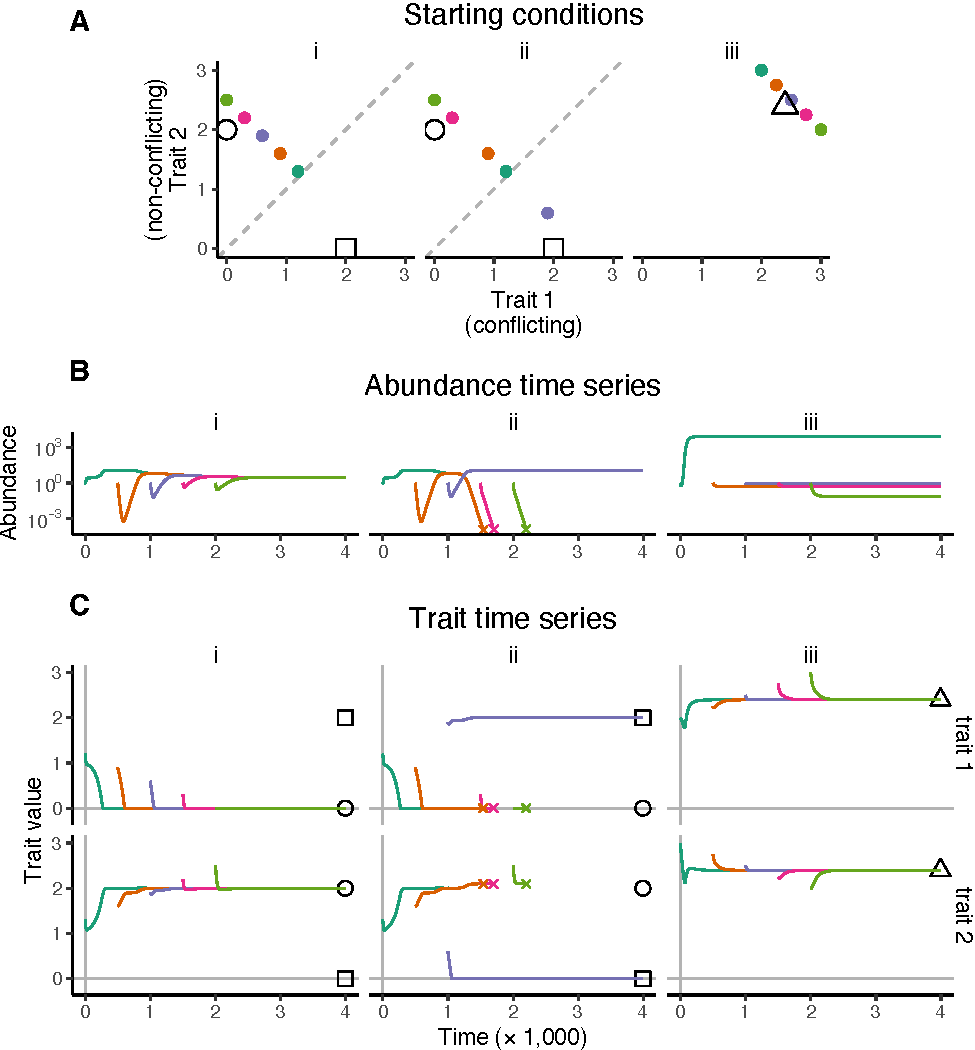
\includegraphics[width=0.7\textwidth]{3-cond_coexist_conflicting.pdf}
\caption{Conditional coexistence for 2-axis, 5-species communities when axis 1 has 
    conflicting evolution and axis 2 has non-conflicting.
    Panels show, for each of five situations,
    (A) starting conditions and trajectories for each species in axis space, 
    (B) abundances through time, and 
    (C) axis values through time.
    Situation i has sub-additive tradeoffs, situations ii and iv have 
    super-additive, and iii and v have additive.
    (A) Dashed arcs show the location of neutrally stable rings
    when tradeoffs are additive, and 
    the dotted lines separate the basins of attraction for the two possible
    axis states when tradeoffs are super-additive.
    (A,C) Shapes of hollow points indicate the equilibrium axis state.
    (C) For situations iii and v, line width is proportional to the 
    distance from the neutrally stable ring.
    Xs mark extinction events.
}
\label{fig:conditional-coexistence}
\end{figure}


The outcomes of these simulations changed somewhat when we included stochasticity
into these simulations.
Stochasticity in abundance decreased coexistence across nearly all situations
(Figure \ref{fig:conditional-coexistence-stoch}A).
The exception was situation ii, which resulted in all 5 species coexisting 
in all simulations for both axis and abundance stochasticity
(Figure \ref{fig:conditional-coexistence-stoch}A,B).
For situations iv and v, where coexistence did not occur in deterministic
simulations, abundance stochasticity changed nothing.

Like population stochasticity, axis stochasticity had a strong negative 
effect on coexistence for situations i and iii but had no effect on
situation iv (Figure \ref{fig:conditional-coexistence-stoch}B).
For situation v, however, axis stochasticity allowed for coexistence
when deterministic simulations resulted in exclusion, 
and it resulted in different species surviving.
This is because the axis stochasticity caused species to evolve 
along the ring (towards the center) instead of staying in place once they 
reached it (Figure \ref{fig:cond-coexist-Vstoch-sit-v}).
[[NOTE: Could this be because the error term is log-normal, so its mean is
$> 1$ and causes both axes to increase??]]
This resulted in the first two species being ``better equipped'' to evolve in 
response to the invader that is closer to the conflicting axis being
maximized.
It also caused the invader to evolve away from maximizing the conflicting
axis, which reduced its ability to exclude the others.



\begin{figure}[ht!]
\centering
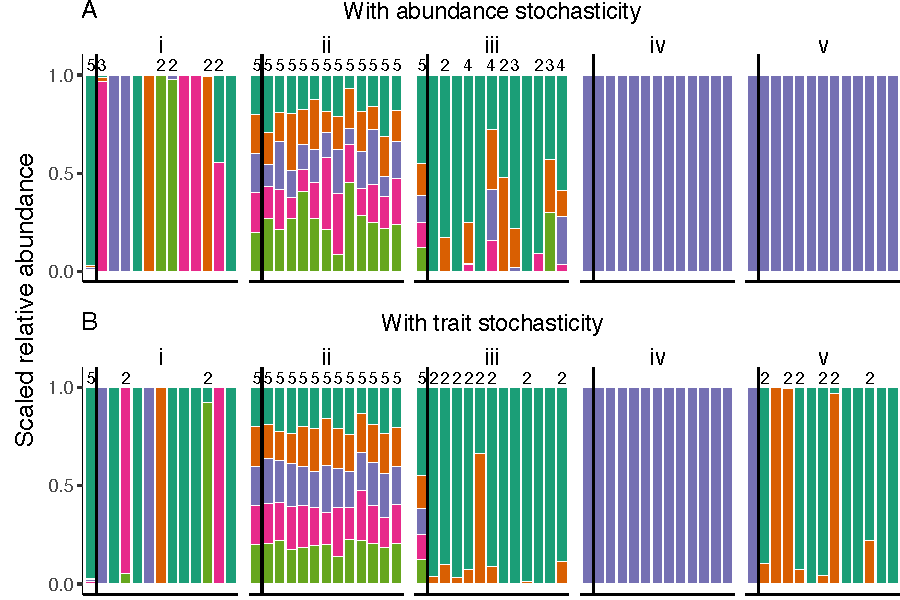
\includegraphics{4-cond_coexist_stoch.pdf}
\caption{Outcomes from stochastic simulations of 2-axis, 5-species communities 
    when axis 1 has conflicting evolution and axis 2 has non-conflicting.
    Panels show scaled relative abundance(s)
    ($\sqrt{N_i} \, / \, \sum_k^n{\sqrt{N_k}}$) 
    of surviving species for simulations with
    (A) abundance stochasticity ($\sigma_N = 0.1$) and
    (B) axis stochasticity ($\sigma_V = 0.1$).
    Each bar in each sub-panel represents a simulation repetition.
    Bars to the left of the black vertical lines are for when there was no 
    stochasticity.
    Small numbers above bars indicate the number of species that coexisted
    when coexistence occurred.}
\label{fig:conditional-coexistence-stoch}
\end{figure}



To explore the effect of axis evolution stochasticity on coexistence across 
the axis space,
we simulated a one-species equilibrium community that was invaded by 
a species that varied in its starting axis values.
We compared the probability of coexistence with stochasticity to that without.
We found a largely negative effect across much of the axis space
(Figure \ref{fig:inv-sims-heatmap-coexist}).
The exception was in marginal starting axis values, where some locations
had drastic improvements in coexistence probability---0 in deterministic 
simulations and 1 in stochastic simulations.
The range where improvements occurred varied with $d_1$ and with tradeoff type.
Additive tradeoffs showed no areas where stochasticity helped coexistence.

\begin{figure}[ht!]
\centering
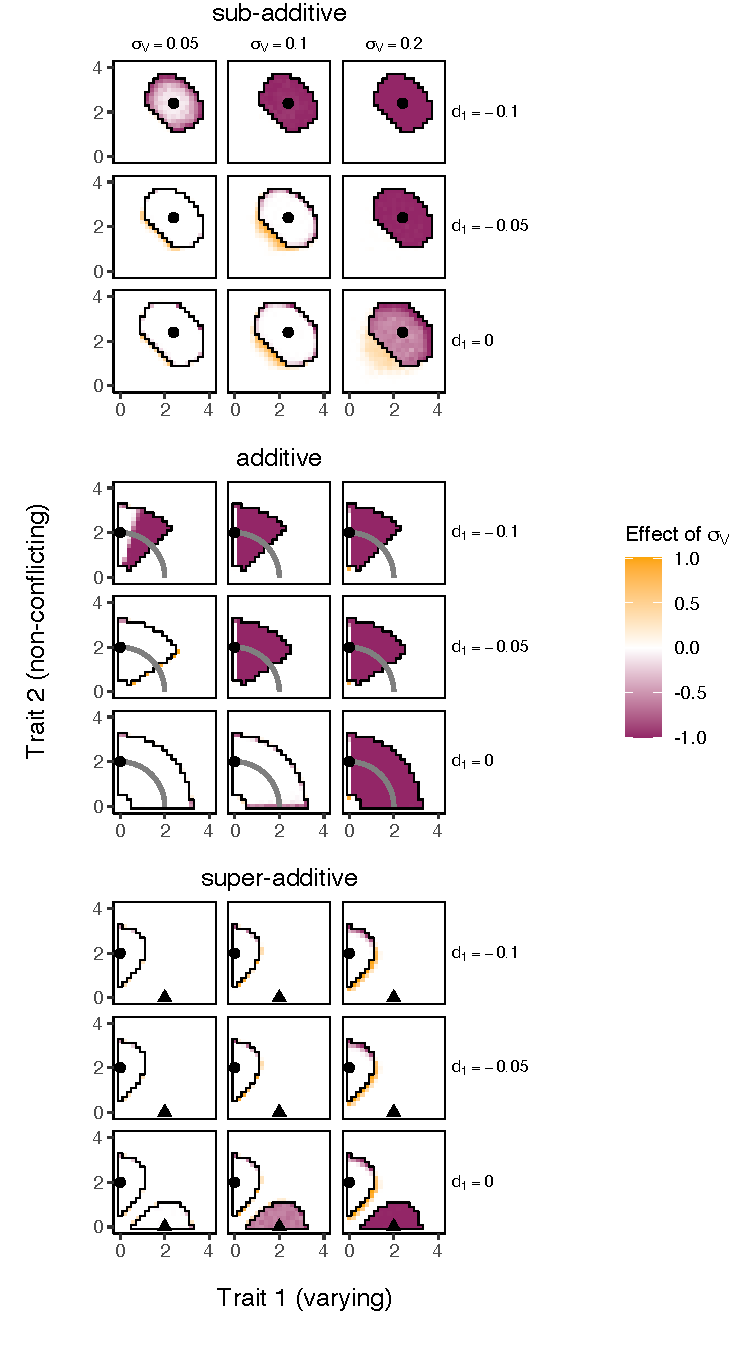
\includegraphics[width=0.5\textwidth]{5-inv_sims_hm_coexist.pdf}
\caption{Effect of stochasticity on coexistence of a resident species and 
    an invader based on the invader's starting axis values (x and y axes),
    magnitude of stochasticity (sub-panel columns), and 
    value of $d_1$ (sub-panel rows).
    The fill color of each cell indicates how much stochasticity changed
    the probability of coexistence compared to deterministic simulations,
    and white indicates no effect.
    Round points indicate the axis values of the resident species,
    triangle points indicate an alternative stable equilibrium state, 
    and a gray line indicates a neutrally stable ring.
    The area of the heatmap outlined by a thin, black line is where
    coexistence occurred in deterministic simulations.
    For these simulations, $d_2 = 0.1$ and $\sigma_i = 0.05$.
    Shown for sub-additive, additive, and super-additive tradeoffs.}
\label{fig:inv-sims-heatmap-coexist}
\end{figure}
